\chapter{Tinjauan Pustaka}
\label{bab:02}

Bab ini berisi ilmu dan konsep yang mendukung pem bahasan tesis ini beserta
makalah mengenai pekerjaan sebelumnya dalam deteksi vandalisme di Wikipedia.
Untuk konsep sampel ulang yang dibahas adalah metode \textit{Synthetic Minority
Oversampling Technique} (SMOTE) dan ekstensi dari SMOTE yaitu
\textit{Local Neighbourhood SMOTE} (LNSMOTE).
Konsep pengklasifikasi yang dibahas dan digunakan yaitu \textit{Random Forest}
(RF) dan ekstensinya yaitu \textit{Cascaded Random Forest} (CRF).

	\section{SMOTE}
	\label{bab:02:smote}
	Metode \textit{Synthetic Minority Over-sampling Technique} (SMOTE)
\parencite{chawla2002smote} menggunakan pendekatan \textit{over-sampling} yang mana
kelas minoritas ditambah dengan membuat sampel sintetis, bukan dengan
mengganti sampel dari kelas mayoritas menjadi kelas minoritas.
Sampel sintetis dibuat lewat aplikasi dengan beroperasi pada
ruang fitur.
Kelas minoritas ditambah dengan mengambil setiap sampel-sampel dari kelas
minoritas dan membuat sampel sintetis di antara segmen garis yang menghubungkan
setiap $k$ tetangga terdekat (\textit{k-nearest-neighbors}, KNN) dari kelas
minoritas.
Instan dari KNN dipilih secara acak, bergantung dari jumlah
\textit{over-sampling} yang dibutuhkan.

\begin{figure}[htbp]
\centering
\setlength\fboxsep{4pt}
\fbox{
	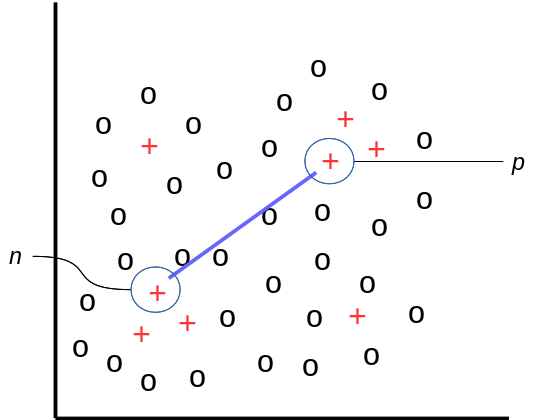
\includegraphics[keepaspectratio=true,scale=0.35]{SMOTE-example}
}
	\caption{
	Ilustrasi pembuatan sampel sintetis pada SMOTE.
	Misalkan $p$ adalah sampel minoritas dan $n$ adalah salah satu dari $k$
	tetangga terdekat dari $p$, maka
	sampel sintetis yang baru akan berada di garis antara $p$ dan $n$.
	}
	\label{fig:smote}
\end{figure}

Sampel sintetis dibuat dengan cara berikut, misalkan $p$ adalah salah satu
sampel minoritas pada dataset $D$,
\pagebreak
\begin{itemize}
	\item Cari $k$ sampel tetangga dari $p$ pada $D$
	\item Untuk setiap sampel tetangga $k$,
	\begin{itemize}
		\item Hitung selisih antara vektor fitur $p$ dengan tetangga $k_{i}$
		\item Kalikan selisih tersebut dengan angka ril acak antara 0 sampai 1,
		dan
		\item simpan hasilnya ke vektor fitur sintentis yang baru.
	\end{itemize}
\end{itemize}

Cara ini membuat sampel secara acak pada segmen garis antara dua fitur yang
terpilih, seperti yang terlihat pada gambar \ref{fig:smote}.
Pendekatan ini secara efektif mendorong wilayah pembelajaran dari kelas
minoritas menjadi lebih besar tanpa menyebabkan \textit{overfitting}.


	\section{LNSMOTE}
	\label{bab:02:lnsmote}
	Meskipun hasil SMOTE dibuktikan bagus dalam makalah Chawla dkk.
\cite{chawla2002smote}, metode ini masih memiliki beberapa kelemahan.
Pertama, cara menentukan sampel minoritas sebagai calon untuk
\textit{over-sampling} bisa bermasalah.
Pada SMOTE, semua sampel dari kelas minoritas digunakan.
Namun, bukan berarti semua sampel tersebut sama bergunanya bagi pembelajaran
klasifikasi.
Pada khususnya, sampel yang ada pada batas \textit{decision}, atau berada
dibatas kelas minoritas dengan kelas mayoritas, lebih sering salah
diklasifikasi dibandingkan dengan sampel yang berada jauh dari batas kelas,
oleh karena itu mereka lebih penting untuk klasifikasi.
Sampel yang jauh dari batas kelas, berada di tengah kelas minoritas mungkin
berkontribusi sedikit pada klasifikasi.
Salah satu metode untuk menangani permasalahan ini yaitu dengan hanya
mengambil sampel pada batas kelas minoritas yang dijadikan untuk
\textit{oversampling}, seperti yang diajukan oleh Han dkk.
\cite{han2005borderline} dengan menggunakan metode bernama \textit{Borderline
SMOTE}.

\begin{figure}[htbp]
	\centering
	\begin{subfigure}[b]{0.4\textwidth}
		\centering
		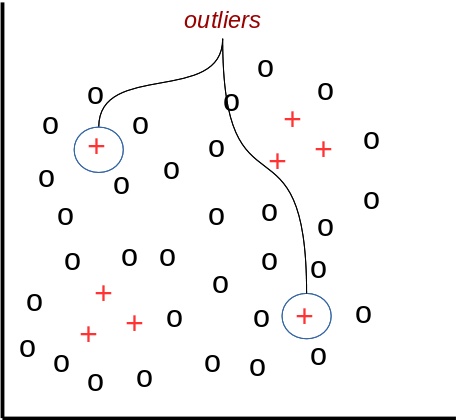
\includegraphics[width=\textwidth]{SMOTE-problem-outliers}
		\caption{}
		\label{fig:smote-outliers}
	\end{subfigure}
	\begin{subfigure}[b]{0.5\textwidth}
		\centering
		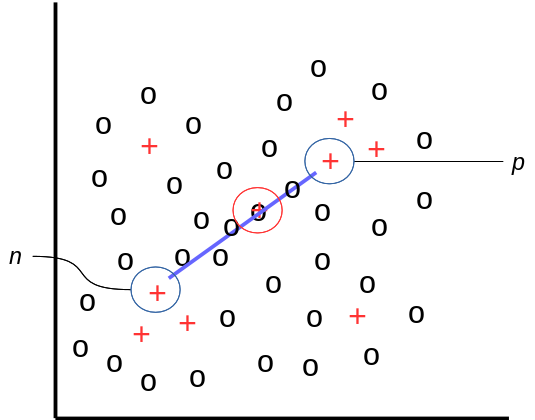
\includegraphics[width=\textwidth]{SMOTE-problem-overlapping}
		\caption{}
		\label{fig:smote-overlapping}
	\end{subfigure}
	\caption{
Kelemahan metode SMOTE:
(a) \textit{Outliers} pada kelas minoritas tidak diperhitungkan pada metode
SMOTE.
(b) Pembuatan sampel sintetis yang baru berada di wilayah kelas mayoritas
yang tumpang-tindih dengan sampel kelas mayoritas.
	}
	\label{fig:smote-problems}
\end{figure}

Kelemahan lain dari SMOTE yaitu permasalahan \textit{overgeneralization} yang
begitu saja menggeneralisasi wilayah dari kelas minoritas.
SMOTE tidak mempertimbangkan distribusi dari sampel pada kelas mayoritas, atau
adanya \textit{outliers}.

Untuk mengatasi permasalahan di atas, Maciejewski dkk. memperkenalkan ekstensi
dari metode SMOTE bernama \textit{Local-neighbourhood SMOTE} atau disingkat
LNSMOTE \cite{maciejewski2011local} yang menggunakan modifikasi dari
pendekatan \textit{Safe-Level SMOTE} \cite{bunkhumpornpat2009safe}.
Pada metode \textit{Safe-level SMOTE} keberadaan sampel mayoritas
diperhitungkan sebelum membuat sampel sintetis dengan menghitung sebuah
koefisien khusus yang disebut \textit{safe level}.
Untuk setiap sampel dari kelas minoritas, dihitung jumlah sampel kelas
minoritas di antara \textit{k-nearest-neighbors} (KNN).
Jika nilainya sama atau mendekati $ 0 $, sampel tersebut dianggap sebagai
\textit{noise}.
Jika nilainya mendekati $ k $, maka sampel tersebut bisa dikatakan berada
di wilayah aman dari kelas minoritas.
Gagasan utamanya adalah membuat sampel sintetis yang dekat dengan wilayah aman.

Lebih rincinya, misalkan $ p $ adalah sampel dari kelas minoritas yang akan
menjadi calon untuk \textit{over-sampling}, maka $ k $ sampel terdekat dengan
$ p $ yang termasuk pada kelas minoritas $ P $ ditentukan.
Seperti pada SMOTE, setidaknya satu dari tetangga tersebut dipilih, sebutlah
dengan $ n $.
Untuk kedua sampel, $ p $ dan $ n $, $ k $ sampel terdekatnya untuk keseluruhan
data pelatihan $ S $ dihitung \textit{safe level}-nya dengan notasi $ sl(p) $
dan $ sl(n) $.
Dari pengetahuan tersebut, koefisien rasio \textit{safe-level} ditentukan
dengan $ \textit{sl-ratio} = sl(p) / sl(n) $.
Langkah selanjutnya ditentukan berdasarkan 5 kasus berikut:
\begin{enumerate}
	\item \label{case:safe-1} Jika $ sl(p) = 0 $ dan $ sl(n) = 0 $, sampel
	$ p $ dan $ n $ dianggap sebagai \textit{noise outliers}, dan tidak ada
	sampel sintetis yang dibuat.
	\item Jika $ sl(p) > 0 $ dan $ sl(n) = 0 $, maka $ n $
	adalah \textit{noise}.
	Sampel sintetis akan dibuat jauh dari $ n $ dengan menduplikasi $ p $.
	\item Jika $ sl-ratio = 1 $, maka $ p $ dan $ n $ memiliki tetangga
	yang sama dan sampel sintetis yang baru akan dibuat diantara garis yang
	menghubungkan mereka dengan cara yang sama seperti pada SMOTE.
	\item Jika $ sl-ratio > 1 $, maka $ p $ berada di wilayah
	aman minoritas daripada $ n $ dan sampel sintetis yang baru akan
	dibuat dekat dengan $ p $, dengan parameter acak pada SMOTE akan
	memiliki rentang $ [0, 1 / \textit{sl-ratio}] $.
	\item Jika \textit{sl-ratio < 1}, maka \textit{n} berada di wilayah
	aman minoritas daripada $ p $ dan sampel sintetis yang baru akan
	dibuat dekat dengan $ n $, yaitu parameter acak pada SMOTE akan
	memiliki rentang $ [1 - \textit{sl-ratio}, 1] $.
\end{enumerate}

Strategi \textit{safe-level SMOTE} bermasalah khususnya pada distribusi kelas
yang bias yang mana kelas minoritas menyebar sehingga terdiri dari beberapa
sub-wilayah dengan kardinalitas yang kecil.
Situasi ini mengacu pada permasalahan yang disebut \textit{small disjuncts}
yang diakui sebagai sumber kesulitan yang paling penting bagi pembelajaran
klasifikasi untuk data timpang \cite{jo2004class}.
Pada kasus seperti ini pembuatan sampel sintetis dengan \textit{Safe-level
SMOTE} bisa menyebabkan terjadinya tumpang-tindih antara kelas.

Sebagai contohnya, misalkan dua kelompok dari kelas minoritas terpisah
dikelilingi oleh sampel dari kelas mayoritas.
Katakanlah, jarak antara kedua kelompok minoritas tersebut cukup jauh, satu
kelompok berada di bawah dan kelompok lainnya di atas.
Misalkan calon dari sebuah sampel berada di kelompok yang dibawah.
Jika parameter $ k $ dari fungsi pencarian KNN lebih besar dari jumlah sampel
kelas minoritas di dalam kelompok tersebut, maka tetangga dari kelas minoritas
selanjutnya akan menjadi sampel dari kelompok yang lain.
Jika rasio \textit{safe-level} dari sampel kedua kelompok sama, sampel sintetis
yang baru bisa dibuat diantara garis yang menggabungkan sampel-sampel dari
kedua kelompok tersebut.
Dengan kata lain, sampel sintetis yang baru bisa berada di wilayah yang dihuni
oleh kelas mayoritas.
Makanya, strategi ini masih memungkinkan terjadinya tumpang-tindih antara
kelas.

Situasi tidak diinginkan seperti di atas disebabkan karena teknik SMOTE mencari
KNN yang dimiliki oleh kelas minoritas saja.
Jika calon sampel tidak berada di wilayah yang padat dengan kelas minoritas,
maka beberapa tetangganya bisa saja cukup jauh dan juga sampel dari kelas
mayoritas mengelilingi calon sampel tersebut.

LNSMOTE mengatasi masalah tumpang tindih ini dengan lebih mempertimbangkan
tetangga sekitar
(\textit{local neighbourhood})
dari calon sampel minoritas yang mungkin bisa memberikan perkiraan dari
keberadaan sampel kelas mayoritas.
Jadi, pencarian sampel yang terlalu jauh sebaiknya dihindarkan.

Modifikasi teknik LNSMOTE terhadap \textit{Safe-Level} SMOTE yaitu,
\begin{itemize}
\item jika calon sampel $ p $ diidentifikasi berada di tetangga terdekat $ k
$ dari $ n $, sampel tersebut tidak langsung dihitung dengan $ sl(n) $ tapi
dicari tetangga dari $ k + 1 $ selanjutnya.
\item Membatasi rentang interval di mana sampel baru secara acak ditempatkan.
Jadi, pada beberapa kasus dari \textit{safe-level}, LNSMOTE tidak menentukan
batas kanan dari interval dengan 1 tapi sebagai ambang batas $\tau < 1$.
Ambang batas tersebut tidak baku tapi ditentukan secara dinamis bergantung
kepada \textit{safe-level} dari sampel mayoritas.
\item Jika $ sl(n) $ relatif rendah, artinya $ n $ dikelilingi oleh banyak
sampel dari kelas mayoritas, sampel baru seharusnya ditempatkan lebih dekat ke
$ p $.
\item Jika $ n $ dikelilingi oleh sejumlah sampel minoritas yang seimbang,
sehingga nilai $ sl(n) $ tinggi, sampel yang baru bisa berada di dekat $ n $.
Hal ini supaya bisa mengontrol tingkat ekspansi dari kelas minoritas dengan
cara dinamis, memperhitungkan distribusi lokal dari sampel.
\end{itemize}

Algoritma LNSMOTE yang digunakan pada implementasi tesis berdasarkan pada
makalah Maciejewski dkk.
\cite{maciejewski2011local}
yang dapat dilihat pada lampiran
\ref{lampiran:alg_lnsmote}.


	\section{\textit{Random Forest}}
	\label{bab:02:rf}
	\textit{Random Forest} (RF) \cite{breiman2001random}
adalah sebuah kombinasi dari beberapa pohon keputusan yang mana setiap pohon
bergantung kepada nilai dari vektor acak yang disampel secara independen dan
dengan distribusi yang sama.

Pohon keputusan yang digunakan dalam RF dapat menggunakan ID3
(\textit{Iterative Dichotomiser}), C4.5 (pengganti dari ID3), atau CART
(\textit{Classification and Regression Trees}).
Dalam tesis ini, dan umumnya pada implementasi RF, menggunakan CART sebagai
pohon keputusan.

Ada tiga parameter utama dalam pembentukan RF.
Parameter pertama yaitu jumlah pohon yang akan dibangun dalam \textit{forest}
(katakanlah $n$),
parameter kedua yaitu persentase dari sampel pelatihan yang digunakan untuk
membangun pohon (katakanlah $b$),
dan parameter ketiga yaitu jumlah fitur acak yang juga digunakan untuk
membangun pohon (katakanlah $m$).
Ketiga parameter diatur sebelum memulai pembangunan RF dan nilainya sama untuk
semua pohon.

Persentase dari sampel pelatihan yang diambil secara acak umumnya dua per tiga
dari sampel keseluruhan, sehingga meninggalkan sepertiganya sebagai
\textit{out-of-bag} (OOB).
Untuk nilai acak fitur $m$, nilai yang biasa digunakan yaitu akar dari jumlah
fitur atau $log$ dari jumlah fitur \cite{breiman2001random}.

Proses pembangunan RF sebagai berikut.
Diasumsikan diberikan sebuah dataset latihan $S$.
Setelah parameter ditentukan, pada saat pembuatan pohon, ambil sampel dari $S$
secara acak tanpa diganti (sampel yang telah diambil bisa terpilih kembali pada
pengambilan acak berikutnya) sejumlah $b$.
Proses ini dikenal juga dengan \textit{bootstraping}.
Sampel yang tidak terpilih disebut dengan \textit{out-of-bag} (OOB), yang
bisa digunakan untuk penghitungan laju galat mis-klasifikasi.
Dari sampel yang terpilih tersebut ambil $m$ buah fitur secara acak, kemudian
bangun pohon dari $m$ fitur dan $b$ sampel acak tersebut tanpa dibersihkan
(\textit{pruning}).
Ulangi proses tersebut sampai pohon ke-$n$.

Proses klasifikasi pada RF berjalan seperti berikut.
Diberikan dataset $T$ yaitu dataset yang berisi fitur yang sama dengan dataset
pelatihan $S$.
Untuk setiap sampel yang akan diklasifikasi pada dataset $T$, masukan sampel
tersebut ke setiap pohon.
Kumpulkan hasil klasifikasi dari setiap pohon, kemudian ambil mayoritas kelas
dari semua hasil klasifikasi tersebut.
Fungsi selengkapnya dari pembuatan dan klasifikasi RF dapat dilihat pada
algoritma \ref{alg:rf}.

\begin{center}
\captionof{algorithm}{Random Forest}
\label{alg:rf}
	\begin{algorithmic}[1]
\Require \\
$ TSET $: dataset pelatihan \\
$ T $: jumlah pohon untuk \textit{forest} \\
$ B $: persentase sampel yang dipilih secara acak tanpa diganti dari $TSET$ \\
$ m $: jumlah fitur acak \\

\Function{RandomForest}{$ TSET, T, B, m $}
	\State $ n \gets $ jumlah sampel pada dataset $ TSET $
	\State $ b \gets n * (B / 100) $
	\Comment Jumlah sampel untuk setiap pohon.

	\State $ forest \gets nil $
	\For{$ t \gets 1,T $}
		\State $ tp, tn, tree \gets \Call{GrowTree}{forest, TSET, b, m} $
		\State $ \Call{forest.Add}{tree} $
	\EndFor
	
	\State \Return $forest$
\EndFunction
\\
\Function{GrowTree}{$ forest, TSET, b, m $}
	\label{bagging}
	\State $ bag, oob, bagIdx, oobIdx \gets \Call{RandomPickSample}{$ TSET,
	b $} $

	\State $ tree \gets \Call{BuildTree}{bag, m} $

	\State $ \Call{forest.SaveBagIndex}{bagIdx} $
	\Comment Simpan pohon dan indeks dari \textit{bagging}

	\State $ cm \gets \Call{Classify}{forest, oob, oobIdx} $
	\State $ tp, tn \gets \Call{ComputeStat}{cm} $
	\Comment Hitung laju galat OOB dari \textit{confusion matrix}
	$cm$.

	\State \Return{$ tp, tn, tree $}
\EndFunction
\\
\Function{Classify}{$ forest, set, setIdx $}
	\State $ predictions \gets nil $
	\For{\textbf{each} $ sample, idx $ \textbf{in} $ set $}
		\State $ votes \gets \Call{ForestVotes}{forest, sample, idx} $
		\State $ class \gets \Call{Majority}{votes} $
		\Comment ambil mayoritas suara kelas pada $votes$
		\State $ predictions.push(class) $
	\EndFor

	\State \Return $predictions$
\EndFunction
\\
\Function{ForestVotes}{$ forest, sample, idx $}
	\State $ votes \gets nil $
	\For{\textbf{each} $ tree $ \textbf{in} $forest$ }
		\State $ exist \gets \Call{IsSampleInTheBag}{idx} $
		\Comment Periksa apakah sampel indeks digunakan pada pohon ini.

		\If{exist}
			\State continue
			\Comment Jika digunakan, lanjutkan ke pohon berikutnya.
		\EndIf

		\State $ class \gets \Call{tree.Classify}{sample} $

		\State $ \Call{votes.push}{class} $
	\EndFor

	\State \Return $ votes $
\EndFunction
	\end{algorithmic}
\end{center}



	\section{\textit{Cascaded Random Forest}}
	\label{bab:02:crf}
	Permasalahan umum dalam penggalian data atau algoritma pembelajaran ansambel
adalah ketidakmampuan untuk menangani data pelatihan yang timpang.
Ketimpangan antara kelas positif dan negatif biasanya menyebabkan akurasi
deteksi yang rendah.
Simulasi yang dilakukan oleh Strobel dkk. \cite{strobl2007bias} menampilkan
bahwa RF condong mendukung kelas mayoritas.
Saat menggunakan RF untuk deteksi, sejumlah besar sampel negatif dibutuhkan
untuk mendapatkan pengklasifikasi yang kuat dan laju \textit{false-positive}
yang rendah.
Hal ini menyebabkan ketimpangan yang besar antara kelas positif dan
negatif, sehingga membuat pengklasifikasi RF yang berfokus pada kelas
mayoritas.
Kelemahan lain dari RF yaitu setelah belajar dengan beberapa pohon, RF secara
gradual mencapai titik puncaknya, yang mana pengklasifikasi tidak bisa lagi
meningkatkan \textit{sensitivity} pada pendeteksian maupun mengurangi laju
\textit{false-positive}-nya.

Pada tahun 2011, Viola dan Jones mengajukan algoritma deteksi sampel cepat
berbasis AdaBoost dengan struktur kaskade (\textit{cascade})
\cite{viola2004robust}.
Struktur kaskade dimotivasi oleh asumsi bahwa lebih mudah untuk menolak sebuah
sampel yang negatif daripada mencari sampel yang positif.
Viola dan Jones menggabungkan pengklasifikasi yang kuat pada beberapa tingkatan
yang independen dengan kondisi bahwa setiap tingkat dapat menolak sebuah
sampel, sehingga supaya sebuah sampel dapat dianggap positif semua tingkat
harus terlewati.
Disebabkan karena dominasi penolakan pada tahap-tahap awal, waktu komputasi
menjadi berkurang.
Sebagai tambahan, untuk mendapatkan pelatihan yang lebih baik, Viola dan Jones
mengajukan strategi \textit{bootstrap} dengan menghapus sampel yang benar
terklasifikasi negatif setelah pembelajaran dilakukan pada setiap tingkat.
Setelah itu, dataset pelatihan yang berkurang ditambahkan dengan sampel yang
salah diklasifikasi (\textit{false-positive})
\cite{viola2004robust}.

Sebuah pengklasifikasi kaskade terdiri dari sejumlah tingkatan dengan
kompleksitas yang meningkat.
Setiap tingkat minimum memiliki satu pengklasifikasi independen.
Pengklasifikasi ditambahkan ke dalam tingkatan sampai batas nilai
\textit{true-positive} dan \textit{true-negative} tercapai.
Keuntungan dari struktur kaskade yaitu sejumlah besar sampel dapat
didistribusikan diantara tingkatan, berkurangnya nilai \textit{false-positive},
dan berkurangnya waktu komputasi baik pada pelatihan dan klasifikasi.

Baumann menerapkan metoda ini pada RF dan mengajukan \textit{Cascaded Random
Forest} (CRF) yaitu penggabungan dari pengklasifikasi RF dengan struktur
kaskade, yang menyusun beberapa pohon keputusan dalam setiap tingkatan dengan
strategi agregasi \textit{bootstrap}.
Sehingga, pembelajaran pada sampel positif meningkat dan kelemahan dari data
yang timpang terhindari \cite{baumann2013cascaded}.

Pengklasifikasi CRF memiliki enam parameter umum, tiga diantaranya sama dengan
RF yaitu jumlah pohon ($T$), persentase sampel acak untuk \textit{bootstrap},
($b$), dan jumlah fitur acak ($m$).
Tiga parameter lainnya yaitu jumlah tingkatan ($S$), nilai ambang batas
\textit{true-positive} ($maxtp$), dan nilai ambang batas
\textit{true-negative} ($maxtn$).

Strategi \textit{bootstrap} yang digunakan adalah sebagai berikut: setelah
menyelesaikan pembelajaran pada sebuah tingkatan, dataset pelatihan yang berisi
hanya sampel negatif diujikan ke semua tingkatan yang telah dibentuk
sebelumnya dengan tujuan untuk menghapus sampel yang benar bernilai
\textit{true-negative} saja, sehingga dataset pelatihan sebisa mungkin berisi
hanya sampel positif.
Sampel yang terklasifikasi \textit{false-positive} kemudian dimasukan kembali
ke dataset pelatihan untuk dipelajari oleh tingkatan berikutnya.
Fungsi selengkapnya dari CRF dapat dilihat pada algoritma \ref{alg:crf}.

Beberapa tingkatan memiliki akurasi deteksi yang lebih rendah daripada
yang lainnya.
Untuk mengurangi pengaruh tingkatan yang memiliki performansi yang rendah
tersebut, maka dihitung faktor bobot $\alpha$ dari setiap tingkatan dengan
mengeksploitasi rerata harmonik dari \textit{precision} dan \textit{recall},
atau dikenal juga dengan nilai $F_1$ (\textit{fmeasure}),
pada dataset pelatihan.

Nilai $\alpha$ pada setiap tingkatan secara linear dinormalisasi pada rentang 0
dan 1, sehingga bobot dari tingkat yang memiliki performansi yang rendah
berkurang supaya pengaruhnya terhadap mayoritas \textit{voting} juga berkurang.
Proses untuk mendapatkan hasil dari pengklasifikasi CRF diberikan pada gambar
\ref{form:crf}.

\begin{figure}[h]
\[
	y(x) = argmax \left(
			\frac{1}{T \cdot \sum^{S}_{s=1} \alpha_{s} }
			\sum\limits_{s=1}^{S} \alpha_{s}
			\sum\limits^{T}_{t=1} I_{h_{t} (x) = c}
		\right)
\]
\caption{
Formula untuk mendapatkan kelas (\textit{voting}) pada pengklasifikasi CRF
dengan bobot.
}
\label{form:crf}
\end{figure}

Pada gambar \ref{form:crf}, $x$ adalah sampel yang akan diklasifikasi,
$S$ adalah jumlah tingkatan pada struktur kaskade,
$\alpha_{s}$ adalah nilai bobot dari tingkatan,
$T$ adalah jumlah pohon pada tingkatan, dan
$h_{t}$ yaitu fungsi klasifikasi dari sebuah pohon yang memberikan sebuah nilai
kelas $c$ yang bisa memiliki nilai indikator dari $I$
(misalkan nilai 1 untuk positif atau 0 untuk negatif).


	\section{Pekerjaan Terkait}\label{bab:02:pekerjaan_terkait}
	Deteksi vandalisme di Wikipedia berbasis pendekatan pembelajaran mesin telah
menjadi topik penelitian yang menarik sejak tahun 2008.
\textcite{potthast2008automatic} berkontribusi untuk pendekatan deteksi
vandalisme dengan pembelajaran mesin yang pertama, dengan menggunakan fitur
tekstual berikut fitur meta data dasar dengan menggunakan pengklasifikasi
\textit{logistic regression}.
\textcite{smets08automaticvandalism} menggunakan pengklasifikasi Naive Bayes
pada sekumpulan kata yang merepresentasikan suntingan dan yang pertama
menggunakan model kompresi untuk mendeteksi vandalisme di Wikipedia.
\textcite{itakura2009using} menggunakan Kompresi Markov Dinamis
untuk mendeteksi suntingan vandalisme di Wikipedia.
\textcite{mola2012wikipedia} mengembangkan pendekatan yang dilakukan
oleh \textcite{potthast2008automatic} dengan menambahkan beberapa fitur
tekstual dan berbagai fitur berbasis daftar-kata.
Velasco memenangi \textit{1st International Competition on Wikipedia Vandalism
Detection}.
\textcite{west2011multilingual} adalah yang pertama
mengajukan pendekatan deteksi hanya berdasarkan meta data
spasial dan temporal, tanpa perlu memeriksa teks pada artikel dan revisi.
\textcite{adler2010detecting} membangun sebuah sistem deteksi vandalisme
menggunakan sistem reputasi WikiTrust.
\textcite{adler2011wikipedia} kemudian menggabungkan bahasa alami,
spasial, temporal, dan fitur reputasi yang digunakan pada karya sebelumnya.
\textcite{west2011multilingual} adalah yang pertama memperkenalkan
data \textit{ex post facto} sebagai fitur, yang mana perhitungannya
mempertimbangkan revisi selanjutnya.
Sistem deteksi vandalisme West dan Lee memenangkan \textit{2nd International
Competition on Wikipedia Vandalism Detection}.
\textcite{harpalani2011language} menyatakan suntingan vandalisme
memiliki properti lingustik yang unik dan sama.
Harpalani dkk. membangun sistem deteksi vandalisme berdasarkan analisis
\textit{stylometric} dari suntingan vandalisme dengan model probabilitas
\textit{context-free grammar}.
Pendekatan Harpalani dkk. mengalahkan sistem berbasis fitur dengan pola
dangkal, yang menyamakan struktur sintaksis dan token teks.
Mengikuti tren dari klasifikasi vandalisme antar bahasa,
\textcite{tran2013cross} mengevaluasi berbagai pengklasifikasi berbasiskan pada
sekumpulan fitur independen bahasa yang dikumpulkan dari jumlah artikel dilihat
setiap jam dan riwayat suntingan Wikipedia.

\textcite{gotze2014advanced} menggabungkan fitur dari
\textcite{adler2011wikipedia},
\textcite{javanmardi2011vandalism},
\textcite{mola2012wikipedia},
\textcite{potthast2008automatic},
\textcite{wang2010got}, dan
\textcite{west2011multilingual} dengan empat fitur tambahan dan perubahan.
Untuk mengatasi masalah ketimpangan pada korpus,
\textcite{gotze2014advanced}
mengaplikasikan teknik
\textit{random oversampling}
bernama
\textit{Synthetic Minority Over-sampling TEchnique} (SMOTE)
yang diajukan oleh
\textcite{chawla2002smote},
dan kombinasi dari SMOTE dan
\textit{random undersampling}.
Dataset latihan yang orisinal dan hasil sampel ulang diuji dengan
pengklasifikasi satu-kelas dan dua-kelas.
Pengklasifikasi satu-kelas yang diterapkan diantaranya
\textcite{hempstalk2008one}
dan SVM oleh
\textcite{scholkopf1999support}
yang diimplementasikan oleh
\textcite{chang2011libsvm}
pada korpus PAN-WVC.
Pengklasifikasi dua-kelas yang diterapkan diantaranya
\textit{Logistic Regression},
\textit{RealAdaBoost},
\textit{Random Forest} (RF), dan
\textit{Bayesian Network}.
Hasil percobaan yang didapat memperlihatkan performansi pengklasifikasi
satu-kelas tidak kompetitif dengan satu pun pengklasifikasi dua-kelas.
Hal ini bisa disebabkan karena tidak sesuainya kelompok fitur yang digunakan
untuk menjelaskan suntingan vandalisme, sebagaimana juga parameter pengaturan
yang tidak sesuai pada pendekatan yang digunakan.
Hasil dari pelatihan pada dataset orisinal memperlihatkan RF
lebih unggul dari pengklasifikasi lainnya.
Hasil dari pelatihan pada dataset hasil sampel ulang memperlihatkan adanya
peningkatan pada semua pengklasifikasi kecuali pada RF.



Dari penelitian di atas, tujuh diantaranya menggunakan PAN-WVC-10
\parencites{adler2010detecting}
{adler2011wikipedia}
{gotze2014advanced}
{harpalani2011language}
{mola2012wikipedia}
{wang2010got}
{west2011multilingual},
dengan nilai presisi terbaik yaitu $0,86$, nilai \textit{recall} $0,57$, dan
PR-AUC $0,66$ didapat oleh Velasco menggunakan \textit{Random Forest} tanpa
penyeimbangan dataset.
Hanya dua yang menggunakan PAN-WVC-11
\parencites{gotze2014advanced}
{west2011multilingual}
dengan hasil terbaik dipegang oleh Gotze yaitu
dengan nilai presisi $0,92$, \textit{recall} $0,39$, dan PR-AUC $0,74$.

